% ALGUNOS PAQUETES REQUERIDOS (EN UBUNTU): %
% ========================================
% %
% texlive-latex-base %
% texlive-latex-recommended %
% texlive-fonts-recommended %
% texlive-latex-extra %
% texlive-lang-spanish (en ubuntu 13.10) %
% ******************************************************** %

\documentclass[a4paper]{article}
\usepackage[utf8]{inputenc}
\usepackage{fancyhdr}
\usepackage[pdftex]{graphicx}
\usepackage{sidecap}
\usepackage{caption}
\usepackage{subcaption}
\usepackage{booktabs}
\usepackage{makeidx}
\usepackage{float}
\usepackage{array}
\usepackage{amsmath, amsthm, amssymb}
\usepackage{amsfonts}
\usepackage{sectsty}
\usepackage{wrapfig}
\usepackage{listings}
\usepackage{pgfplots}
\usepackage{enumitem}
\usepackage{hyperref}
\usepackage{listings}
\usepackage{listingsutf8}
\usepackage{pgfplotstable}
\usepackage{colortbl}
\usepackage[spanish,es-nodecimaldot]{babel}
\graphicspath{imagenes/}}

\linespread{factor}

\definecolor{mygreen}{rgb}{0,0.6,0}
\definecolor{mygray}{rgb}{0.5,0.5,0.5}
\pgfplotsset{compat=1.3}
\setlist[enumerate]{label*=\arabic*.}
\lstset{
	inputencoding=utf8/latin1,
	language=C++,
	basicstyle=\ttfamily,
	keywordstyle=\bfseries\color{blue},
	stringstyle=\color{red}\ttfamily,
	commentstyle=\color{mygreen}\ttfamily,
	morecomment=[l][\color{magenta}]{\#},
	numbers=left,
	numberstyle=\color{mygray}
}
\pgfplotstableset{% global config, for example in the preamble
  every head row/.style={before row=\toprule,after row=\midrule},
  every last row/.style={after row=\bottomrule},
  fixed,precision=2,
}

\usepackage{color} % para snipets de codigo coloreados
\usepackage{fancybox}  % para el sbox de los snipets de codigo

\definecolor{litegrey}{gray}{0.94}

% \newenvironment{sidebar}{%
% 	\begin{Sbox}\begin{minipage}{.85\textwidth}}%
% 	{\end{minipage}\end{Sbox}%
% 		\begin{center}\setlength{\fboxsep}{6pt}%
% 		\shadowbox{\TheSbox}\end{center}}
% \newenvironment{warning}{%
% 	\begin{Sbox}\begin{minipage}{.85\textwidth}\sffamily\lite\small\RaggedRight}%
% 	{\end{minipage}\end{Sbox}%
% 		\begin{center}\setlength{\fboxsep}{6pt}%
% 		\colorbox{litegrey}{\TheSbox}\end{center}}

\newenvironment{codesnippet}{%
	\begin{Sbox}\begin{minipage}{\textwidth}\sffamily\small}%
	{\end{minipage}\end{Sbox}%
		\begin{center}%
		\vspace{-0.4cm}\colorbox{litegrey}{\TheSbox}\end{center}\vspace{0.3cm}}



\usepackage{fancyhdr}
\pagestyle{fancy}
%\renewcommand{\chaptermark}[1]{\markboth{#1}{}}
\renewcommand{\sectionmark}[1]{\markright{\thesection\ - #1}}
\fancyhf{}
\fancyhead[LO]{Sección \rightmark} % \thesection\
\fancyfoot[LO]{\small{Nicolás Bukovits, Kevin Frachtenberg, Julián Len, Nicolás Len}}
\fancyfoot[RO]{\thepage}
\renewcommand{\headrulewidth}{0.5pt}
\renewcommand{\footrulewidth}{0.5pt}
%\setlength{\hoffset}{-0.8in}
\setlength{\textwidth}{16cm}
\setlength{\hoffset}{-1.1cm}
\setlength{\headsep}{0.5cm}
\setlength{\textheight}{25cm}
\setlength{\voffset}{-0.7in}
\setlength{\headwidth}{\textwidth}
\setlength{\headheight}{13.1pt}
\renewcommand{\baselinestretch}{1.1} % line spacing

\usepackage{caratula}

\newcommand{\ord}{\ensuremath{\operatorname{O}}}
\newcommand{\nat}{\ensuremath{\mathbb{N}}}

\begin{document}

\setcounter{page}{1}
\materia{Algoritmos y Estructuras de Datos III}
\submateria{Segundo Cuatrimestre de 2016}
\titulo{Trabajo Práctico II}
%\subtitulo{Grupo: }
\integrante{Nicolás Bukovits}{546/14}{nicobuk@gmail.com}
\integrante{Kevin Frachtenberg}{247/14}{kevinfra94@gmail.com}
\integrante{Julián Len}{467/14}{julianlen@gmail.com}
\integrante{Nicolás Len}{819/11}{nicolaslen@gmail.com}
\maketitle
% no footer on the first page
\thispagestyle{empty}

\newpage
\tableofcontents

\newpage
\section{Introducción}

En este trabajo se tienen tres problemas que se resolvieron aplicando las
técnicas algorítmicas estudiadas en la materia. Los mismos presentaron cada uno un desafío
distinto, teniendo que aplicar métodos diferentes para resolverlos y cumplir
con los requisitos exigidos.

Además de la resolución de los mismos, se procedió a demostrar la correctitud de
cada implementación. Esto fue acompañado a su vez de una justificación de la
complejidad temporal.

Cada ejercicio contó con su respectiva experimentación para corroborar que la
complejidad temporal teórica se cumpliera y en los casos donde el algoritmo
podía comportarse mejor, verlo reflejado de alguna manera.

Los experimentos contaron con diversas medidas para asegurar su efectividad de
las cuales las siguientes fueron iguales para los tres problemas:
\begin{itemize}
	\item{Sólo se midió el costo temporal de generar la solución, no
			de lectura y escritura del problema.}
	\item{Para la medición del tiempo se utilizó la biblioteca \texttt{chronos}
			con unidad de tiempo en microsegundos.}
\end{itemize}


% \newpage
%  \section{Ejercicio 1: Laberinto}
    % 1. Describir detalladamente el problema a resolver dando ejemplos del mismo y sus soluciones.
    \subsection{Descripción del problema}
		    Indiana Jones continua en su expedición en la fortaleza de alguna civilización antigua. Mientras llenaban las mochilas con los tesoros que más les convenian encontraron un mapa peculiar. El mapa se parece mucho a un laberinto salvo por el hecho de que no estan conectados todos los puntos. En el mapa hay un punto que parece indicar el lugar en donde se encuentran juntando tesoros, y hay un lugar que esta indicado con una cruz. Intrigados por saber lo que se encuentra en ese lugar, se proponen como objetivo ir hacia ahi. Como nuestro equipo vino equipado con pico y pala, pueden derribar algunas paredes. Por otro lado el equipo ya se encuentra cansado y no desea recorrer mucha distancia ni esforzarse rompiendo paredes. Entonces, nos pidieron ayuda con lo siguiente: Teniendo un mapa indicando un punto de origen (identificado con una $o$) y un punto de destino (identificado con una $x$), quieren caminar lo menos posible desde el origen al destino rompiendo a lo sumo una cierta cantidad de paredes.

        La resolución del problema consiste en encontrar el camino más corto que derribe a los sumo $P$ paredes, las cuales se reconocen de un mapa dibujado con $.$ y $\#$ que indican los lugares por donde se puede pasar y las paredes respectivamente. Cada paso cuenta como 1 avance desde el origen y cuando una pared es derribada, se toma en cuenta como un lugar por el que se puede pasar, por lo que suma 1 también como parte del camino. El mapa tiene tamaño $F$ filas y $C$ columnas, los cuales se pasan por parametro al programa junto con la cantidad de paredes y el mapa. En caso de que este camino no exista, entonces la salida será solamente $-1$

        Por ejemplo, si el programa recibe lo siguiente como entrada: \newline
        \texttt{5} \texttt{9} \texttt{2} \newline
        \texttt{\# \# \# \# \# \# \# \# \#} \newline
        \texttt{\# o \# . \# . \# x \#} \newline
        \texttt{\# . \# . \# . \# . \#} \newline
        \texttt{\# . \# . \# . . . \#} \newline
        \texttt{\# \# \# \# \# \# \# \# \#} \newline

        La salida correcta sería: \newline
        \texttt{10}

    % 2. Explicar de forma clara, sencilla, estructurada y concisa, las ideas desarrolladas para la resolución del problema. Utilizar pseudocódigo y lenguaje coloquial (no código fuente). Justificar por qué el procedimiento resuelve efectivamente el problema.
    \subsection{Solución propuesta}
        Este problema resulta más simple de entender cuando se piensa el mapa como un grafo dirigido en tres dimensiones, donde la cantidad de nodos será de $FC(P+1)$ y en cada nivel habrá $FC$ nodos. De esta manera, podemos ver a cada piso del grafo (comenzando en el piso 0) como la cantidad de parades que se rompieron hasta ese punto. Los nodos estarán conectados cada uno con sus vecinos, aunque si uno de ellos es una pared, entonces el nodo se conectará con el vecino que representa a la pared pero un nivel más arriba. Hay que tener en cuenta que los nodos se modelan, para cada nivel, simplemente como el número de nodo en el grafo base (el del nivel 0) más la cantidad de nodos de cada nivel, y sus conexiónes (o aristas) se almacenan en listas de adyacencias.

        Teniendo el mapa representado de esta manera, sabemos en todo momento que la cantidad de paredes derribadas es menor o igual al límite establecido, por lo que si se puede llegar a la $x$ destruyendo una cantidad menor o igual de paredes que $P$, entonces existe un camino entre el origen y el destino.

        Para encontrar el camino mínimo entre $o$ y $x$ utilizamos el algoritmo conocido como \textit{Breadth-first Search} o \textit{BFS}, el cual conciste en recorrer el grafo analizando una sola vez cada nodo y desde éllos, observar sus vecinos. Si los vecinos de ese nodo aún no fueron analizados, se agregan a una cola para ser revisados después. Cada vez que se observa un vecino, chequeamos que no haya sido visto con anterioridad y si ese es el caso, se marca como visto cargando su distancia al origen en una \textit{lista de distancias} y agregándolo a la cola. Este algoritmo funciona en grafos donde las aristas no tienen peso o sus pesos son todos iguales, como en este ejercicio que como se dijo anteriormente, avanzar en el mapa implica sumar 1 a la cantidad de pasos, o bien aumentar en 1 la distancia al origen. Luego, los pesos de las aristas serán todos de valor 1 y puede utilizarse BFS.

        La \textit{lista de distancias} tiene el tamaño de la cantidad de nodos totales y cada posición $i$ representa al nodo $i$ del grafo. Esta lista solamente contiene la distancia al origen de cada nodo, inicializándose con $-1$ para todos y a medida que avanza el algoritmo, si el vecino $k$ del nodo $i$, que es el que se está analizando tiene distancia menor a $0$, entonces quiere decir que aún no ha sido observado.


        \subsubsection{Detalles implementativos}
            Para poder manejar correctamente el grafo, se creó la clase ListaAdy con namespace Grafos, la cual modela un grafo representado con listas de adyacencias. Las únicas operaciones que tiene la clase son el constructor, que recibe la cantidad de nodos totales, agregarArista, que recibe dos enteros $u,v$ y agrega $v$ a la lista de adyacencias de $u$, y BFS que recibe el número de nodo origen $s$, el número de origen de destino $t$, y la cantidad $f$ de filas y $c$ de columnas.
            La forma en que se almacenan las listas de adyacencias es con un vector de vectores de enteros, tipo que se provee de la librería estándar de C++.

            Normalmente, BFS solo necesitaría el nodo de origen y de destino, y almacenaría todos las posibles distancias de caminos que hay entre ambos nodos. Sin embargo, agregamos estos dos valores para el algoritmo termine la primera vez que encuentre el nodo destino. Esto es por cómo funciona BFS: Al recorrer todos los nodos según su distancia al origen, siempre se analizan los nodos que solo están a distancia 1 más que el nodo vecino "padre" (o sea, el nodo que tenía como vecino al que se está analizando y por el cual se agregó a la cola de revisión). Ergo, si existe un camino entre $s$ y $t$, BFS encontrará el más corto antes que cualquier otro y por eso es que podemos terminar su ejecución cuando eso pase. En peor caso, no existirá un camino entre $s$ y $t$, y BFS recorrerá todos los nodos.

            El algoritmo que resuelve el problema puede separarse en dos partes: Una se encarga de leer el mapa de entrada y construir el grafo dirigido tridimensional y la otra, es el BFS que busca verdaderamente la solución.
            En la primera parte recorremos el mapa que se encuentra guardado en una matriz de \textbf{char} $P+1$ veces, para así poder construir los $p+1$ niveles del grafo y poder conectar cada nodo con sus respectivos vecinos, y para poder verificar que el mapa pasado sea válido y buscar los nodos marcados con la $o$ y la $x$.
            La segunda parte se recorre el grafo una sola vez dado el funcionamiento de \textit{BFS}, pero como tiene $FC(P+1)$ nodos, entonces esa será la cantidad de nodos que pasarán por la cola de revisión como máximo. La función BFS está implementada de la siguiente manera:


            \begin{codesnippet}
            \begin{verbatim}
BFS(enteros : s, t, f, c)
  res = -1
  cola = cola vacía
  distancias[nodosTotales]
  para i entre 0 y nodosTotales-1
    distancias[i] = -1
  fin para

  cola.encolar(s)
  distancias[s] = 0
  mientras (cola no esté vacía)
    tope = cola.tope
    cola.desencolar //al ser una cola, desencola el tope de la misma
    si (tope % (f*c)) == t
      devolver distancias[tope]
    fin si

    para i entre 0 y largo(vecinos(tope))
      si distancias[vecinos(tope)[i]] < 0
        distancias[vecinos(tope)[i]] = distancias[tope] + 1
        cola.encolar(vecinos(tope)[i])
      fin si
    fin para
  fin mientras

  devolver res
            \end{verbatim}
            \end{codesnippet}

            El único cambio que tiene esta implementación de BFS respecto de la original, es que chequea si el resultado se encuentra antes de terminar, lo cual puede hacerse por lo antes dicho. Como complemento, podemos decir que en el código puede observarse que $distancias[tope]$ siempre existe y es mayor a $0$ porque antes de agregar un nodo a la cola, se carga en $distancias$ su valor correspondiente. Además, la razón por la cual se chequea el resto de dividir $tope$ por $f*c$ es que t es el número del nodo con la $x$ en el nivel 0, mientras que al ser un grafo tridimensional donde cada nivel representa la cantidad de paredes rotas desde el origen, $t$ va a estar en todos los niveles con una diferencia de $f*c*nivelActual$. Ergo, al dividir tope por $f*c$, el resto debería ser el número de nodo que se va a analizar como si fuera uno del nivel 0.



    % 3. Deducir una cota de complejidad temporal del algoritmo propuesto y justificar por qué el algoritmo cumple la cota dada. Utilizar el modelo uniforme.
    \subsection{Complejidad teórica}

      Para este análisis, nuevamente separaremos el algoritmo en dos partes (construcción del grafo y BFS). En la primera parte, se generan $P+1$ niveles de $FC$ nodos que como se explica en el punto anterior, se representan mediante listas de adyacencias. Agregar una arista entre dos nodos cuesta $O(1)$ ya que es simplemente agregar el número de nodo destino de la arista a la lista de adyacencia del nodo origen. Hacer esto por cada nodo costaría $O(|E|)$ por cada nivel con $|E|$ siendo el número de aristas. Sin embargo, al ser un digrafo tipo \textit{grid}, la cantidad máxima de aristas por nodo es de 4 porque cada nodo se conecta con, a lo sumo, un nodo a cada lado (izquierda, derecha, arriba y abajo). Además, si bien hay $FC$ nodos en cada nivel, los nodos que sean paredes no tendrán aristas de entrada que provengan de nodos del mismo piso. Luego, $|E| \leq 4FC \in O(FC)$. Como esto ocurre $P+1$ veces, la complejidad de la primera parte es

      \[
        O((P+1)FC) \in O(FCP)
      \]


      La segunda parte, el algoritmo conocido como \textit{BFS}, tiene complejidad $O(|V| + |E|)$ siendo $|V|$ la cantidad de nodos. Ya probamos que $|E| \in O(FCP)$ y sabemos que $|V| = FC$, entonces la complejidad de la segunda parte es

      \[
        O(FC + FCP) \in O(FCP)
      \]

      Considerando las dos partes juntas, nos queda que la complejidad temporal es

      \[
        O(FCP + FCP) \in O(FCP)
      \]

      En cuanto a la complejidad espacial, el tamaño del grafo sobre listas de adyacencias es de $O(FCP)$ ya que es la cantidad de nodos totales sumado a lo que, por lo probado anteriormente, acota la cantidad de aristas totales.


    % 4. Dar un código fuente claro que implemente la solución propuesta. Se deben incluir las partes relevantes del código como apéndice del informe impreso entregado.

    % 5. Realizar una experimentación computacional para medir la performance del programa implementado. Usar un conjunto de casos de test en función de los parámetros de entrada, con instancias aleatorias e instancias particulares (de peor/mejor caso en tiempo de ejecución, por ejemplo). Presentar en forma gráfica una comparación entre los tiempos medidos y la complejidad teórica calculada y extraer conclusiones.
    \subsection{Experimentación}

	Para poder mostrar que la cota propuesta en la complejidad temporal funciona para el algoritmo que resuelve este problema, realizamos experimentos con cantidades de personas entre 1 y 7 pero siempre con mayor o igual número de arqueólogos que de caníbales. Los casos de prueba pueden observarse en la tabla que se encuentra en el anexo de este informe.

  Los resultados obtenidos fueron plasmados en el siguiente gráfico. El mismo es la representación del tiempo en funcion de la cantidad de arqueólogos. También se muestra la funcion propuesta como cota de complejidad temporal.

  \begin{figure}[H]
      \begin{center}
        \includegraphics[width=0.7\columnwidth]{imagenes/exp1Ej1-1a7.jpeg}
        \caption{}
      \end{center}
  \end{figure}

  Para cada valor en $x$ puede observarse que a medida que crece, hay más puntos en $y$ para el mismo $x$. Esto es porque si bien el eje X es la cantidad de arqueólogos, también varía la cantidad de caníbales por lo que el tiempo que toma cada ejecución del programa también depende de este valor, pero como se aclaró en la sección de complejidad, el número de caníbales va de 0 a la cantidad de arqueólogos (porque en caso contrario el programa termina en seguida a menos que no haya arqueólogos, caso que se verá más adelante) lo cual implica que nuestro tamaño de entrada $n$ (la cantidad de arqueólogos) es en realidad a lo sumo $2n$, pero en términos de complejidad el $2$ es una constante que podemos sacar.
  De acuerdo a la tabla proporcionada, los pares (arqueólogo, caníbal) que toman más tiempo son \texttt{(1,1), (2,2), (3,2), (4,2), (5,3), (6,3), (7,3)}. Sin embargo, podemos notar como la cota de complejidad cumple, aunque no de manera ajustada, su función para estos experimentos.


  Para el caso en que no haya arqueólogos y solo haya caníbales, esperábamos que la resolución del problema sea más rápida que en los casos que hay más arqueólogos que caníbales. Probamos con cantidades de caníbales entre 1 y 200 y en el próximo grafico se ilustran los resultados de tiempo en función del número de personas.

  \begin{figure}[H]
      \begin{center}
        \includegraphics[width=0.7\columnwidth]{imagenes/exp2Ej1.jpeg}
        \caption{}
      \end{center}
  \end{figure}

  Notamos como el tiempo que toma a mayor cantidad de caníbales sin arqueólogos crece mucho más lento que para los casos con arqueólogos. Esto se debe a que por un lado, las ramas en que cruzan arqueologos no se prueban, sino que solo se intenta que crucen 1 o 2 caníbales. Luego, la cantidad de estados posibles se reduce a 2 veces la cantidad de formas que se pueden distribuir los caníbales en ambos lados del puente (una por cada lado de la linterna), que es igual a $2*(n^2)$; reducimos la cota de complejidad a $O(n $log$ n*2^{n^2})$. El cambio no es muy grande debido a que las cotas no están totalmente ajustadas, pero funcionan para dar una idea del peor caso acotado por arriba.


\newpage

\section{Ejercicio 2: Menos es más}
    % 1. Describir detalladamente el problema a resolver dando ejemplos del mismo y sus soluciones.

	\begin{figure}[ht]
		\begin{center}
			
\includegraphics[width=0.5\columnwidth]{imagenes/balanza.jpg}
			\caption{Equilibro}
		\end{center}
	\end{figure}

	\subsection{Descripción del problema}
	En su destino hacia la cruz en el mapa recorrieron varias salas distintas. Se dieron cuenta que en cada sala se iban encontrando con un fragmento de una tabla con un mansucrito antiguo. Por lo tanto, antes de continuar, quieren juntarlos todos.\par
	A medida que se iban abriendo camino se dieron cuenta que ciertas paredes derribables requerían cierto esfuerzo para
	abrirse. Este esfuerzo será representado por un $n\in{\mathbb{n}}$ donde $n < 10$. Luego, teniendo un mapa de $F*C$ (F = Filas y C = Columnas), donde se indique el $n$ en las paredes derribables, quieren encontrar cual es el mı́nimo esfuerzo que deben hacer para acceder a todas las salas. \par

	Por lo tanto, se deberá pasar por parametro al algoritmo, el mapa con sus paredes y el esfuerzo para romperlas. 
	\newline
	~

	\textbf{Formato de entrada:} La primer lı́nea consta de dos enteros positivos F y C, donde F es la cantidad de filas en el mapa, y C es la cantidad de columnas. Las siguientes F filas contienen C caracteres. Un “.” representa un lugar caminable, los números del 1 al 9 indican el esfuerzo en romper esa pared, un “\#” representa una pared indestructible. Las paredes con más de 2 paredes adyacentes son indestructibles (contendran un “\#”). Las paredes con menos de 2 paredes adyacentes son indestructibles (contendran un “\#”). Dos salas se pueden conectar si existe una pared adyacente a las dos salas que se puede destruir (Es decir, no quedan conectadas si se rompen muchas parede adyacentes). Por último, los bordes del mapa tendrán un “\#”.


	\begin{verbatim}
    F C
    F_1
    ...
    F_n
    \end{verbatim}
    

	~

	\textbf{Salida:} La salida consta de un número indicando el esfuerzo que debe hacer el equipo para acceder a todas las salas. Si no es posible recorrer todas las salas se imprime un −1. La salida tendrá el siguiente formato:\par
	
	\begin{tabular}{ll}
		\texttt{E}
	\end{tabular}


	%DOY UN EJEMPLO

	~

	Se tiene como restricción que $F$ y $C$ está en el siguiente rango: 1$<=$ $F,C$ $<=$ $10^{4}$. La complejidad temporal debe ser a lo sumo $\ord(FC * \log{FC}{})$.

    % 2. Explicar de forma clara, sencilla, estructurada y concisa, las ideas desarrolladas para la resolución del problema. Utilizar pseudocódigo y lenguaje coloquial (no código fuente). Justificar por qué el procedimiento resuelve efectivamente el problema.
    
    \subsection{Solución propuesta}

    \subsubsection{Modelado}

    Para resolver este problema, se pedía encontrar el mínimo esfuerzo, para pasar por todas las salas del mapa. Para esto se usó el algoritmo de Kruskal, cuyo fín es encontrar el \textbf{Arbol Generador Mínimo} dentro de un grafo, cuyo pesos en las aristas sea positivo. En nuestro caso, esto representaría el mínimo esfuerzo, para poder visitar todas las salas. Para poder usar Kruskal, modelamos el problema en grafos. Para esto, se creó una matriz de $F*C$, donde fueron guardados los caractéres del mapa pasados como parámetro de entrada.\par
    Luego se usó esta matríz para generara los nodos y las aristas. Para esto, en principio cada posicion de la matriz es un nodo, numerados según la posición dentro de la matriz ($filaDelNodoActual * cantColumnas + columnaDelNodoActual$). \par
    Una vez generada la matríz, se la vuelve a recorrer, para generar las aristas. Sea nodoActual, el caracter ubicado en la posición de la matríz en la cual estoy queriendo generar una arista,

    \begin{itemize}
    	\item Si nodoActual es “\#”, no hago nada.
    	\item Caso contrario, me fijo si nodoActual es “.” o un número.
    	\begin{itemize}
    			\item Si es un “.”. Se debe fijar en la columna siguiente de la matriz, a este nodo lo llamaremos, nodoVecino.\par
 		   		Si nodoVecino es distinto de “\#”. Genero una arista, cuyo comienzo es el número de nodoActual, su fin es el de nodoVecino, y el peso es 0. Análogo para la posición inmediata dentro de la matriz, de la fila siguiente.
  		  		\item Si es un número. Deberá hacer lo mismo que en el caso anterior. Con la diferencia que, si uno de sus vecinos es también un número, no deberá hacer nada y que solo tendrá un vecino “.”, en la columna inmediata superior o, en la fila siguiente, dentro de la matriz, y cuyo peso de la arista, será el número del nodo.
 			   	\end{itemize}
    \end{itemize} 


    Luego para el siguiente mapa,

       	\begin{figure}[H]
		\begin{center}
			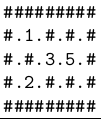
\includegraphics{imagenes/altoMapa.png}
			\caption{Mapa a modelar}
		\end{center}
	\end{figure}


    Queda el siguiente grafo,
    
   	\begin{figure}[H]
		\begin{center}
			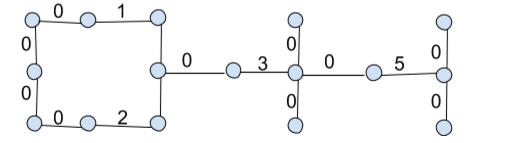
\includegraphics[scale=0.5]{imagenes/grafoOK.png}
			\caption{Grafo del mapa}
		\end{center}
	\end{figure}


    Cada una de estas aristas, es guardada en un vector de aristas.
    Luego, este vector de aristas, es usados como parámetro de entrada, en el algoritmo de Kruskal, quien devolverá la suma del \textbf{Arbol Generador Mínimo}. En caso de no tener solución, es decir, no poder recorrer el mapa, devolverá -1.



	\subsubsection{Implementación}\label{ej2_imp}

	Habiendo introducido la idea, se detalla el comportamiento del algoritmo para
	una entrada arbitraria.


	\begin{enumerate}
		\item{
			La primera parte consiste en la inicialización de valores para el algoritmo. Se guardar la cantidad de filas y de columnas del mapa pasado por standard input. Se crea una matriz con este mismo tamaño. Luego se guardan en esta matriz, los caractéres pasados como parámetros de entrada. Se inicializan valores booleanos para chequear la posibilidad donde no haya solución.
		}

		\item{
			Luego el ciclo principal, consiste en la creación de aristas y nodo. Los nodos serán cada una de las posiciones de la matriz, enumerados desde la posición de la matriz (0,0) hasta (#filas, #columnas).

			Por cada posición recorrida de la matriz se hacen los siguientes chequeos

			\begin{enumerate}
				\item{
					Si matriz[filaActual][columnaActual] es un “\#”, no hago nada.
				}
				\item{
					Caso contrario, si es un “.”:
				}
				\begin{enumerate}
						\item{
							Chequeo matriz[filaActual+ 1][columna] . Si este es distinto de “\#”, creo una arista que empiece desde matriz[filaActual][columnaActual], termine en matriz[filaActual + 1][columnaActual], con peso 0. Lo mismo para matriz[filaActual][columnaActual + 1]. Además aumento la cantidad de nodos y chequeo que el mismo no esté en encerrado, guardando esto en una variable booleana \textbf{encerradoRes}
						}
				\end{enumerate}
				\item{
					Luego, si es un número:
				}
				\begin{enumerate}
						\item{
							Chequeo matriz[filaActual+ 1][columna] . Si este es un “.”, creo una arista que empiece desde matriz[filaActual][columnaActual], termine en matriz[filaActual + 1][columnaActual], con peso igual al número. Lo mismo para matriz[filaActual][columnaActual + 1]
						}
				\end{enumerate}
			\end{enumerate}
			}
			\item{
			    Luego se chequea que hayan más de un nodo o “.”, y en este caso, que no haya ninguno inalcanzable con encerradoRes. Si pasa que no hay nodos, o que si hay más de uno, que alguno esté encerrado, se devuelve -1 (no hay solución).
			}
			\item{
			 	Si la solución es posible, se usa Kruskal con el vector de aristas, quien generará un vector solución de aristas con el \textbf{AGM}. Se sumará el peso de todas las aristas de este vector, para devolver el peso mínimo para recorrer todos los “.” del mapa.
			}
	\end{enumerate}

	\subsubsection{Detalles Implementativos}\label{ej2_det}
		\begin{enumerate}
			\item{
				Para guardar el mapa de parámetro de entrada, se usó una matriz de Char.
			}
			\item{
				Para chequear que un Char es un número válido, se usó la función \textbf{isdigit(char)} perteneciente a la libreryia \textbf{ctype}, y luego se chequeó que el número este entre 1 y 9.
			}
			\item{
				Para guardar las Aristas, se usó la estructura Aristas. La misma contaba con los campos Inicio, Fin y Costo.
			}
			\item{
				Para usar Kruskal, se generó un vector con todas las aristas del grafo.
			}
			\item{
				En Kruskal se usó la estructura de datos \textbf{Union Disjoint Set} (UDS), estructura que cuenta con las operaciones \textbf{find} y \textbf{union}.
			}
		\end{enumerate}


	\subsubsection{Demostración de correctitud}

	Habiendo visto cómo funciona el algoritmo desarrollado, se procede a
	justificar por qué devuelve una solución. Para esto se explicará el algoritmo en base a las justificaciones matemáticas realizadas en la solución propuesta.
	\subsubsection*{Correctitud de ciclo}

	Lo que se va a demostrar a continuación es que el ciclo principal termina y calcula la solución al problema.

	El ciclo se ejecuta mientras P sea distinto de cero. Es decir termina cuando P es 0 y esto ocurre ya que lo que se hace en el ciclo es dividir el número P por 3 y reemplazar P por el resultado (cociente) de esta división en cada iteración. Eventualmente el cociente va a ser cero, por los teoremas de división entera y de desarrollo en base $d$. Lo que se está haciendo es utilizar el algoritmo de división para obtener el desarrollo en base 3 del número $P$. Los restos en cada iteración son los que indican que símbolos hay que utilizar para la representación del número en esa base. En este caso no interesa obtener la representación del número en base 3, sino trabajar con los símbolos en su desarrollo (restos). El resto de la división sólo puede ser 0, 1 o 2 (por el teorema de la división entera).

	A continuación se analiza la parte fundamental del algoritmo que consiste en la identificación de qué pesas utilizar y en qué platillos colocarlas dependiendo del resto. Se tienen las siguientes posibilidades: 

	\begin{enumerate}
		\item{
			Resto == 0. En este caso, si la última pesa fue colocada del lado izquierdo no hay que realizar nada. Esto es porque el anterior dígito en el desarrollo era o bien otro cero o un 1. Por lo tanto no es necesario utilizar esta pesa para compensar una de un valor menor que no pudo ser utilizada porque se estaban usando dos (esto fue explicado en la solución propuesta). En cambio si la anterior pesa fue colocada del lado derecho es porque el anterior dígito en el desarrollo del número era un 2. En este caso, hay que utilizar esta pesa, por lo que se agrega a la lista de izquierdas el valor de la potencia de 3 correspondiente. Independientemente de si se utilizó esta pesa o no, la variable izquierda se actualiza con el valor verdadero, ya que el hecho de que no se use una pesa de una determinada potencia también se toma como que se 'usó'' la pesa de la izquierda. Esto es porque en el caso de que el siguiente dígito en el desarrollo sea un uno, se tiene que poder distinguir si el anterior fue un 0 o un 2, lo cual no se podría realizar si no se actualiza el valor de esta variable. En la explicación del caso del resto 1 se puede entender mejor esta conclusión. 
		}
		\item{
			Resto == 1. En este caso siempre hay que agregar una pesa. Si el valor de la variable izquierda es verdadero (esto es porque el anterior dígito fue un 0 o un 1) hay que agregar esta potencia de 3 a la lista de izquierda. En el caso contrario significa que el anterior dígito era un 2 y como se demostró en la solución propuesta hay que colocar esta pesa en el lado derecho, ya que si el anterior fue un 2 hay que tomar este dígito, lo que lo convertiría de un 1 a un 2, y por lo tanto hay que aplicar nuevamente la fórmula propuesta. Por lo tanto en este último caso se agrega la potencia de 3 correspodiente en la pesa derecha. El valor de la variable izquierda no es necesario actualizarlo ya que si se agrega a la lista de izquierdas hay que modificarlo por verdadero (lo cual ya ocurre porque se agrega solamente a izquierdas si es verdadero) y si se agrega a la lista de derechas hay que modificarlo por falso (lo cual ya ocurre porque se agrega solamente a derechas si es falso).
		}
		\item{
			Resto == 2. En este caso se usa también la idea planteada en la solución al problema. Se agrega a la lista de derechas la pesa con el valor de la potencia de 3 correspondiente solamente si la anterior fue colocada en el lado izquierdo (es decir el anterior dígito es un cero o un uno) ya que si el anterior era un 2 no hay que realizar nada (por lo visto en la demostración de la solución). Finalmente se actualiza el valor de izquierda y se pone en falso siempre, ya que es necesario para el siguiente dígito en el desarrollo, ya que como se vió si el siguiente es cero va a haber que tomar la siguiente pesa y si es un 1 va a haber que colocar la pesa en el lado derecho.	
		}
	\end{enumerate}

	Como el ciclo finaliza cuando P es igual a cero, se puede dar el caso de que el último dígito en el desarrollo del número en base 3 (el más significativo) sea un 2. Por lo tanto y sabiendo que no sigue ningún dígito más, lo que hay que hacer si se da este caso es tomar esta pesa por lo visto en la solución.

	En conclusión lo que hace el algoritmo es dividir iterativamente el número por 3, obteniendo de esta forma su desarrollo en base 3 y al mismo tiempo colocando las pesas correspondientes en base a los restos obtenidos (teorema de desarrollo en base $d$). No es necesario obtener primero la representación del número en la base y después aplicar la solución; se puede realizar mientras se obtiene, tomando decisiones en base al resto de la división en cada iteración. La idea propuesta garantiza que el algoritmo siempre va retornar una solución por lo visto en la sección de "Solución". Las decisiones que se toman con los restos son las inferidas por la solución propuesta: si el dígito es 0, no se toma esa pesa salvo que el anterior sea un 2. si el dígito es 1, si el anterior es 0 o 1 se toma esa pesa, sino se resta la pesa; finalmente si el dígito es 2, si anterior es 2 no se toma ninguna acción y si no se resta la pesa. Además el algoritmo de división garantiza que las pesas que se toman, van a estar ordenadas de menor a mayor cumpliendo con la restricción del problema.

    % 3. Deducir una cota de complejidad temporal del algoritmo propuesto y justificar por qué el algoritmo cumple la cota dada. Utilizar el modelo uniforme.
	\subsection{Complejidad teórica}

	Para calcular la complejidad teórica de la solución propuesta se hará
	referencia a la sección \ref{ej2_imp} donde se posée el pseudocódigo junto a
	su explicación.

	El algoritmo tiene una complejidad temporal de $\ord(log(n))$, por lo tanto es
	logarítmico y cumple con la restricción de complejidad del enunciado. Esto se justifica con el hecho de que el algoritmo posee un ciclo
	principal que se ejecuta mientras $P$ sea distinto de cero, es decir desde el número $P$ hasta el número 0. En cada iteracion el tamaño de $P$ se reduce a un tercio, ya que se divide por 3. Por lo tanto el ciclo se ejecuta la cantidad de símbolos necesarios para obtener el número $P$ en base 3. Si $P$ requiere de $n$ símbolos es que:

	\newline
	$d^{n-1} <= P < d^n$

	\newline
	es decir, $n -1 <= log_3(P) < n$, lo que implica que $[log_3(P)] = n - 1$ y por lo tanto $n = [log_3(P)] + 1$


	Dentro del ciclo sólo se hacen comparaciones que tienen un costo asociado de $\ord(1)$, una división, una multiplicación y una resta de enteros (costo $\ord(1)$), una asignación y una suma, y se agregan elementos a una lista (todas estas operaciones tambien en $\ord(1)$). Por lo tanto se concluye que la complejidad del ciclo es $\ord(log(n))$. Fuera del ciclo sólo se realizan incializaciones de variables $\ord(1)$ al principio del algoritmo y una comparación e inserción en una lista al final también en $\ord(1)$. Por álgebra de órdenes de funciones, la complejidad temporal resultante del algoritmo es $\ord(log(n))$. 

    % 4. Dar un código fuente claro que implemente la solución propuesta. Se deben incluir las partes relevantes del código como apéndice del informe impreso entregado.

    \subsection{Experimentacion}
         

	Se realizaron pruebas experimentales para verificar que el tiempo de
	ejecución del algoritmo cumpliera con la cota asintótica de $\ord(log(n))$,
	demostrada teóricamente. Para ello fue necesario modificar el algoritmo propuesto, ya que como la complejidad está definida por la cantidad de símbolos necesarios para la representación del número en base 3 y se explicó que la misma era $log_3$ del número más uno, no se observan grandes diferencias en el tiempo de ejecución para números 'razonables', es decir números que puedan ser representados de una forma práctica y eficiente en C++. Por ejemplo para el caso de un número muy grande como $3^{30}$, la cantidad de iteraciones que va a realizar el ciclo es sólo 31, que no es muy diferente a la cantidad de iteraciones necesarias para el número $3^{3}$ (4 iteraciones) que es mucho menor. Los tiempos de ejecución de estas instancias son muy similares y dado a que hay muchas variables en cuestión cuando se corren (otros procesos que interfieren, atención de interrupciones y scheduling del S.O, etc) puede hasta darse el caso de que tarde más una instancia menor que una mayor. Se presenta la siguiente modificación del algoritmo para realizar las pruebas:

	\begin{codesnippet}
	\begin{verbatim}
	izquierda = verdadero
	divisiones = 0
	izquierdas = []
	derechas = []
	Mientras v.size != 0
	    Si v[size -1] = 0
	      Si no lo puse en izquierda al anterior
	        Agrego a izquierdas la pesa con valor (3 ^ divisiones)
	      izquierda = verdadero
	    Si v[size -1] = 1
	      Si anterior lo puse en izquierda
	        Agrego a izquierdas la pesa con valor (3 ^ divisiones)
	      Si no
	        Agrego a derechas la pesa con valor (3 ^ divisiones)
	    Si v[size -1] = 2
	      Si anterio lo puse en izquierda
	        Agrego a derechas la pesa con valor (3 ^ divisiones)
	      izquierda = falso
	    v.size -= 1
	    divisiones += 1
	Fin Mientras
	Si el último no lo puse en la izquierda
	   Agrego a izquierdas la pesa con valor (3 ^ divisiones)
	\end{verbatim}
	\end{codesnippet}

	Este algoritmo a diferencia del original, recibe como parámetros un arreglo de enteros (v) que representa el desarrollo en base 3 de un número y un entero que es el tamaño del arreglo. El arreglo de enteros puede contener por lo tanto en cada posición un entero entre 0 y 2 inclusive. El arreglo se interpreta como que en la posición 0 está el dígito más significativo y en la última el menos significativo.
	Con esta idea se puede realizar un mejor análisis del rendimiento del algoritmo ya que se pueden simular números mucho más grandes. Se puede tomar un arreglo de 5000 posiciones, lo cual representaría un número muy grande en base 3 que no se puede representar directamente. La idea es que este algoritmo realiza en el fondo lo mismo que el anterior, ya que lo que se hace es recorrer el arreglo (ciclo principal) y después tomar las mismas decisiones que en el original en base a los valores contenidos en cada posición del arreglo. Es decir lo que determina la complejidad en este caso es el tamaño del arreglo, pero el mismo por lo expuesto anteriormente es igual al logaritmo en base 3 de un número P cualquiera, el cual sería el resultante de realizar la descomposición del desarrollo.

	Para las pruebas lo que se realizó es probar con arreglos de tamaño 1 hasta 4600. Para estandarizar y que no haya constantes diferentes para cada arreglo (ya que lo que se hace depende del valor de cada posición) en todos los casos se completaron todas las posiciones de los arreglos con el valor 1, para que el tiempo esté determinado sólo por el tamaño del arreglo. Además cada uno de los arreglos es testeado 5000 veces para disminuir los outliers. Lo esperable es que haya una relación lineal entre el tiempo de corrida y el tamaño del arreglo, pero el mismo se debe interpretar como que la relación es logarítmica entre el número que representa el arreglo y el tiempo.Se utilizó para que esto se visualice mejor la escala logarítica, como se puede observar en el siguiente gráfico:  


    \renewcommand\constante{5}

	\begin{figure}[H]
      \begin{center}
        \includegraphics[width=0.7\columnwidth]{imagenes/ejercicio2.jpg}
        \caption{}
      \end{center}
  \end{figure}

El análisis expuesto de los datos recopilados presenta evidencia empírica sobre la cota de complejidad
demostrada teóricamente. Además se logra ver que la complejidad depende estrictamente de la cantidad
de símbolos que hay que utilizar para el desarrollo del número en base 3.

% \newpage
% \section{Ejercicio 3: Escapando}

  \begin{figure}[H]
    \begin{center}
      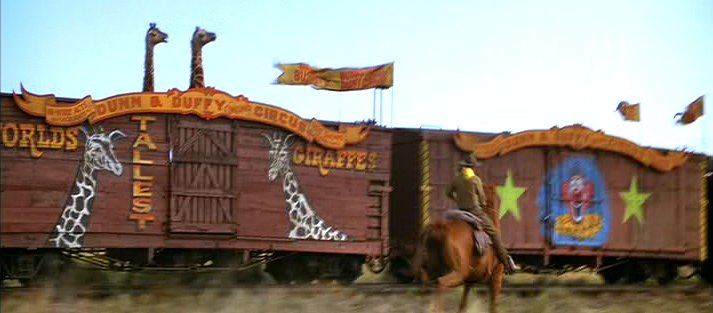
\includegraphics[width=0.4\columnwidth]{imagenes/tren.jpg}
      \caption{El tren se va}
    \end{center}
  \end{figure}


    % 1. Describir detalladamente el problema a resolver dando ejemplos del mismo y sus soluciones.
    \subsection{Descripción del problema}

        \par Luego de colectar todas las piezas Indy se encuentra conforme con lo obtenido, aunque todavía no comprende lo que dice, el material encontrado lo ayudará a conseguir subsidios para continuar con la investigación.
        \par Ya se encuentran en el lugar donde estaba la cruz en el mapa, hay unos carritos sobre vias que parecen dirigirse hacia afuera de la fortaleza. De repente se escuchan unos ruidos muy fuertes desde adentro del laberinto. Luego de romper todas las paredes internas buscando las partes de la tabla se dieron cuenta que se esta desplomando toda la estructura, por lo que deben hacer un escape rápido. \par Al lado del carrito se encuentra un gráfico con la red de las vias. Hay puntos numerados que parecen indicar lugares donde los carritos pueden hacer paradas (estaciones). La estación 1 es donde se encuentran, y la última estación es donde quieren llegar. Las estaciones estan unidas con vías. Al lado de cada vía hay flechas con un número indicando el tiempo que tarda en moverse entre dos estaciones.
        \par Ayudemos a escapar cuanto antes a todos antes de que mueran aplastados.
        \\~\\
        \textbf{En resumen...}
        \par Dado una cantidad de estaciones y una cantidad de vías que cada una conecta un par de estaciones con cierta duración, se debe encontrar la forma más rápida de llegar de la primera a la última estación.
        \\~\\
        \textbf{Formato de entrada:} El formato de entrada contiene dos numeros. La cantidad de estaciones N, y la cantidad de vı́as M. Luego siguen M lı́neas, cada una contiene tres enteros A, B y C que indican que ir de A a B tarda C segundos. Las estaciones estan númeradas de 1 a N.
        
        \begin{verbatim}
        N M
        A_1 B_1 C_1
        ...
        A_M B_M C_M
        \end{verbatim}
        
        \textbf{Formato de salida:} La primera lı́nea deberá tener un entero T indicando el mı́nimo tiempo para ir de la estación 1 a la estación N. Si no es posible, devolver −1. En caso de que sea posible, la segunda lı́nea deberá tener un entero S indicando la cantidad de estaciones que debe recorrer y la tercera lı́nea contendrá S enteros que indican la forma de escapar lo más rápido posible.
        
        \begin{verbatim}
        T
        S
        E_1 E_2 ... E_S
        \end{verbatim}
        
        \textbf{Ejemplos:}
        
        1)
        Una posible entrada válida sería:
        
        \begin{verbatim}
        N = 5   M = 5
        [A B C] = { 1 2 1, 2 3 4, 3 4 5, 4 5 3, 2 4 2 }
        \end{verbatim}

        Y su salida válida sería:

        \begin{verbatim}
        T = 6   S = 4
        E = { 1 2 4 5 }
        \end{verbatim}

        2)
        Otra posible entrada válida sería:
        
        \begin{verbatim}
        N = 6   M = 9
        [A B C] = { 1 2 8, 1 3 4, 2 4 2, 2 5 1, 3 5 1, 4 5 1, 5 4 10, 4 6 1, 5 6 7 }
        \end{verbatim}

        Y su salida válida sería:

        \begin{verbatim}
        T = 11  S = 4
        E = { 1 2 4 6 }
        \end{verbatim}

        3)
        Otra posible entrada válida sería:
        
        \begin{verbatim}
        N = 3   M = 2
        [A B C] = { 1 2 1, 2 1 1 }
        \end{verbatim}

        Y su salida válida sería:

        \begin{verbatim}
        T = -1
        \end{verbatim}


    % 2. Explicar de forma clara, sencilla, estructurada y concisa, las ideas desarrolladas para la resolución del problema. Utilizar pseudocódigo y lenguaje coloquial (no código fuente). Justificar por qué el procedimiento resuelve efectivamente el problema.
    \subsection{Solución propuesta}
    
    \par Como solución decidimos modelar el problema en un grafo y usar el \emph{Algoritmo de Dijkstra} para obtener el camino mínimo de manera tal que no supere la complejidad pedida.

    \par Las estaciones y los recorridos serán modelados en un grafo en el cual los vértices representarán a las estaciones, las aristas representarán a las vías, y el peso de cada arista representará al tiempo que se tarda en llegar de una estación a la otra.
    \par Este grafo será implementado con una lista de adyacencia. Es decir, una lista de N posiciones, siendo N la cantidad de estaciones. Cada posición i tendrá una lista con las estaciones vecinas alcanzables desde la estación i. Cada estación vecina j será una tupla de dos valores: el número de la estación j y el tiempo que se tarda en llegar desde la estación i a la estación j.
    
     \\~\\
     
    \begin{algorithmic}
    \State \Comment {O(m)}
    \Function{Grafo ListAdy}{Int estaciones, Int vias, Lista(estacion1, estacion2, distancia) recorridos}
        \State $listAdy \gets estaciones * \{\}$ \Comment {O(1)}
        \For{$rec \in recorridos$} \Comment {O(m)}
            \State $listAdy_{rec.estacion1}.agregar((rec.estacion2, rec.tiempo))$ \Comment {O(1)}
        \EndFor
        \State \Return {$listAdy$}
    \EndFunction
    \end{algorithmic}
     
     \\~\\
    
    \par Luego se implementará el algoritmo de Dijkstra sobre esta lista de adyacencia. Es decir, siendo N la cantidad de estaciones, el algoritmo resolverá de manera eficiente como llegar de la estación 1 a la N de la forma más rápida.
    \par El algoritmo de Dijkstra recorre los nodos en el orden de distancia al origen. El siguiente nodo a visitar lo elige como el más cercano al origen que no haya sido visitado anteriormente. Y al visitar un nodo actualiza la distancia de sus vecinos y sus respectivos precedentes.
    
     \\~\\
    
    \begin{algorithmic}
    \State \Comment {O((n+m) * $\log n$)}
    \Function{Dijkstra}{Grafo listAdy, Int cantEstaciones}
        \State $time\gets cantEstaciones * \infty$ \Comment {O(n)}
        \State $antecesores\gets cantEstaciones * \infty$ \Comment {O(n)}
        \State $noVisitados\gets ColaDePrioridad((tiempo, estacion))$ \Comment {O($\log n$)}
        \State $time_{0}\gets 0$ \Comment {O(1)}
        \State $noVisitados.encolar((0,0))$ \Comment {O($\log n$)}
        \While {$noVisitados$ tenga elementos} \Comment {O((n+m) * $\log n$)}
            \State $estacion\gets noVisitados.extraerMin()$ \Comment {O($\log n$)}
            \For{$vecino \in listAdy[estacion]$} \Comment {O(m * $\log n$)}
                \If {$time_{vecino} > time_{estacion} + tiempo_{vecino, estacion}$} \Comment {O(1)}
                    \State $nuevoTiempo\gets noVisitados.actualizarPrioridad()$ \Comment {O($\log n$)}
                    \State $time_{vecino}\gets nuevoTiempo$ \Comment {O(1)}
                    \State $antecesores_{vecino}\gets estacion$ \Comment {O(1)}
                \EndIf
            \EndFor
        \EndWhile
        \State \Return {$time_{cantEstaciones}, obtenerSalida(antecesores)$} \Comment {O(n)}
    \EndFunction
    \end{algorithmic}
    
     \\~\\
    
    \par  Para este caso en particular, el algoritmo usará un árbol binario para almacenar los nodos no visitados. De esta manera, se podrá extraer el nodo más cercano al origen y actualizar la prioridad de un nodo cuando se encuentre una distancia menor en complejidad logarítmica.
    \par Para que la función devuelva lo pedido, se obtiene el tiempo mínimo que se tarda en llegar de la estación inicial a la estación final con el valor de la última posición de la lista \emph{time}. Y por otro lado, a partir de la lista \emph{antecesores} se obtiene el recorrido más rápido, con sus estaciones.

    \par El problema planteado se puede visualizar como un contexto en el cual se tiene un grafo con varios vértices (estaciones), con distintas aristas (vías), cada una con su peso (tiempo en llegar de una estación a la otra). Y a partir de este grafo, se desea obtener el camino mínimo desde el primer nodo hasta el último.
    \par Según los algoritmos vistos en la cátedra, la mejor solución para este tipo de problemas es aplicar a ese grafo el \emph{Algoritmo de Dijkstra}, el cual resuelve eficientemente el camino con menos peso para llegar de cierto nodo inicial a cierto nodo final.
    \par Dado este análisis del problema, se llega la conclusión de que el procedimiento desarrollado es una solución eficiente que lo resuelve.
   
    \subsection{Complejidad teórica}
        Dada la explicación anterior, el algoritmo tiene complejidad temporal de $O((N+M) * \log N)$ donde $N$ es la cantidad de estaciones y $M$ es la cantidad de vías.
        Esto se da debido a que se usa el algoritmo de Dijkstra con una lista de prioridad implementada con un árbol binario.
        Notar que $O((N+M) * \log N)$ puede ser peor $O(n^{2})$. Conviene usar min heap o un árbol cuando el grafo es esparso, es decir, cuando M es mucho menor que N^{2}.
    

    % 4. Dar un código fuente claro que implemente la solución propuesta. Se deben incluir las partes relevantes del código como apéndice del informe impreso entregado.

    % 5. Realizar una experimentación computacional para medir la performance del programa implementado. Usar un conjunto de casos de test en función de los parámetros de entrada, con instancias aleatorias e instancias particulares (de peor/mejor caso en tiempo de ejecución, por ejemplo). Presentar en forma gráfica una comparación entre los tiempos medidos y la complejidad teórica calculada y extraer conclusiones.
    \subsection{Experimentación}

        Al igual que con los otros dos ejercicios, se realizaron pruebas experimentales para verificar que el tiempo de ejecución del algoritmo cumpliera con la cota asintótica de $O((N+M) * \log N)$, teóricamente demostrada para el peor caso...
        \par Se plantearon los siguientes casos relevantes para verificar su funcionamiento:
        \par - Se corrieron casos aleatorios alterando la cantidad de vértices, aristas y pesos de cada arista.

        En la siguiente figura, se puede observar los resultados de correr la experimentación explicada. Se muestra el tiempo de procesamiento en función de los vértices...

        \begin{figure}[H]
          \begin{center}
            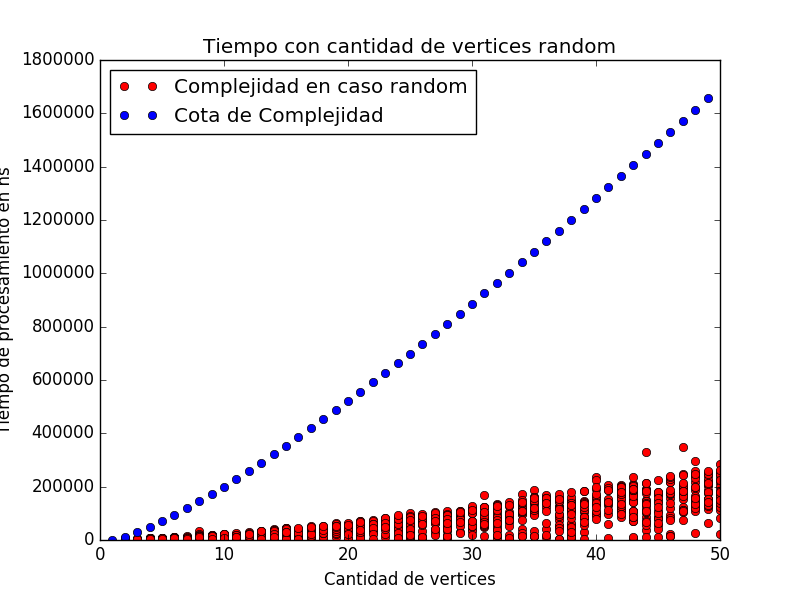
\includegraphics[width=0.7\columnwidth]{../exp/ej3casosRandomVertices.png}
            \caption{}
          \end{center}
        \end{figure}

        En la siguiente figura, se puede observar los resultados de correr la experimentación explicada. Se muestra el tiempo de procesamiento en función de las aristas...

        \begin{figure}[H]
          \begin{center}
            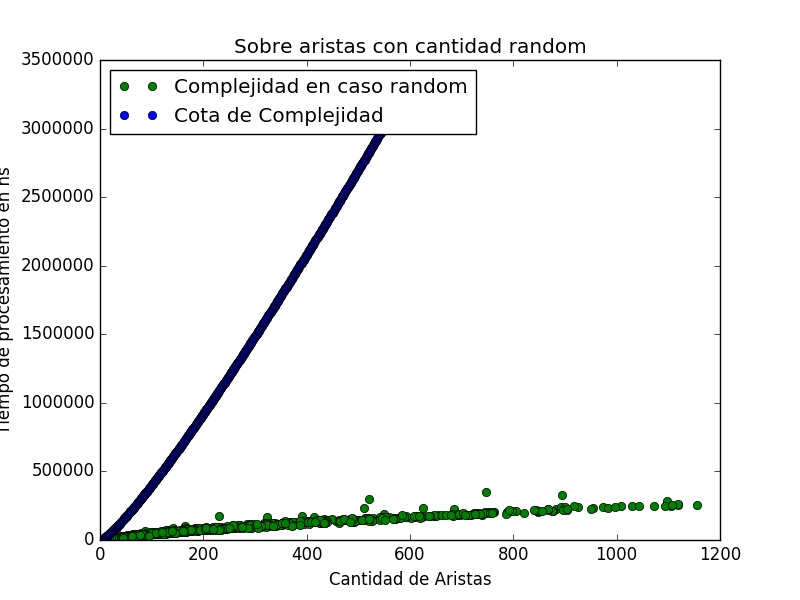
\includegraphics[width=0.7\columnwidth]{../exp/ej3casosRandomAristas.jpeg}
            \caption{}
          \end{center}
        \end{figure}

        Se puede visualizar que los resultados obtenidos en los experimentos con entradas aleatorias difieren mucho con respecto a la cota de complejidad teórica. Esto se debe a que los casos no fueron suficientemente grandes como para alcanzarla. 
        También se puede observar en el gráfico que el tiempo de ejecución no depende únicamente de la cantidad de vértices dado que un grafo puede ser muy denso y esto daría al Algoritmo de Disjktra muchas más posibilidades para recorrer que en el caso en el que hayan pocas aristas. Por eso en el gráfico de tiempo en función de aristas se ven los puntos agrupados en una pendiente creciente, y en el gráfico de tiempo en función de vértices puntos más dispersos.

        \par - Se corrieron casos particulares en los que se debería alcanzar la cota de complejidad. Es decir, los peores casos.
        Para esto, se probó con grafos de n vértices. Para cada vértice i (1 $\leq$ i $<$ n), existe todas las posibles aristas (i, j) tal que j pertenece al intervalo (i, n). Y luego un arista (n-1, n). 
        De esta manera el algoritmo tendrá que recorrer todos los vértices para obtener el camino mínimo.

        \par - Se corrieron casos particulares en los que la complejidad debería ser la mínima posible, es decir, los mejores casos.
        Para esto, se probó con grafos en los que únicamente existía un arista que unía el primer vértice con el último.

        En la siguiente figura, se puede observar los resultados de correr la experimentación explicada...

        \begin{figure}[H]
          \begin{center}
            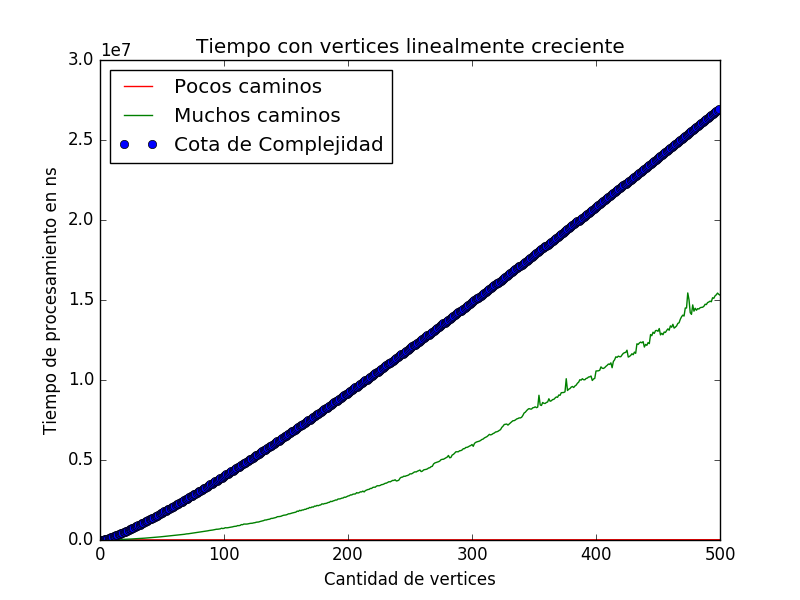
\includegraphics[width=0.7\columnwidth]{../exp/ej3tamanosFijos.png}
            \caption{}
          \end{center}
        \end{figure}

        Se puede visualizar para los peores casos una curva creciente que tiende a la cota de complejidad. Esto se debe a que el Algoritmo de Dijkstra recorre todos los caminos posibles para llegar al último vértice.
        En cambio en el peor caso, como existe una única arista que recorrer, el Algoritmo de Dijkstra encuentra trivialmente el único caso posible. En este caso, lo único que le pesa a la complejidad es la construcción de la lista de adyacencia.

        Cada uno de estos casos consta de entre 500 y 1000 entradas diferentes, y para cada una de esas entradas, se ejecuta el algoritmo 50 veces. En cada una de estas 1000 pruebas se calcula el tiempo promedio (el tiempo de cada ejecución, sobre 50).

        Conclusión: Como se podrá observar realmente el algoritmo para diversos casos cumple la cota dada en la sección de complejidad teórica. También se puede observar que el algoritmo de Dijkstra lo que chequea son las aristas, es decir, la diferencia de la cantidad de aristas es lo que realmente pesa en el tiempo de ejecución para el algoritmo.

\newpage
\appendix
\section{Apéndice}\label{sec:codigo}

\subsection{Tabla de tiempos del Ejercicio 1}

\begin{table}[H]
\centering
\caption{My caption}
\label{my-label}
\begin{tabular}{llll}
\hline
\multicolumn{1}{|l|}{\textbf{Tiempo en ns}} & \multicolumn{1}{l|}{\textbf{Nro Arqs}} & \multicolumn{1}{l|}{\textbf{Nro Cani}} & \multicolumn{1}{l|}{\textbf{Total personas}} \\ \hline
60283                                       & 1                                      & 1                                      & 1                                            \\
72174                                       & 2                                      & 1                                      & 1                                            \\
73101                                       & 2                                      & 2                                      & 2                                            \\
244089                                      & 3                                      & 1                                      & 1                                            \\
376942                                      & 3                                      & 2                                      & 2                                            \\
140744                                      & 3                                      & 3                                      & 3                                            \\
1015891                                     & 4                                      & 1                                      & 1                                            \\
4779930                                     & 4                                      & 2                                      & 2                                            \\
1451661                                     & 4                                      & 3                                      & 3                                            \\
90518                                       & 4                                      & 4                                      & 4                                            \\
3699654                                     & 5                                      & 1                                      & 1                                            \\
89181072                                    & 5                                      & 2                                      & 2                                            \\
100932180                                   & 5                                      & 3                                      & 3                                            \\
1998558                                     & 5                                      & 4                                      & 4                                            \\
115257                                      & 5                                      & 5                                      & 5                                            \\
12750260                                    & 6                                      & 1                                      & 1                                            \\
1380760800                                  & 6                                      & 2                                      & 2                                            \\
12017366000                                 & 6                                      & 3                                      & 3                                            \\
1024082800                                  & 6                                      & 4                                      & 4                                            \\
2600562                                     & 6                                      & 5                                      & 5                                            \\
135313                                      & 6                                      & 6                                      & 6                                            \\
66468300                                    & 7                                      & 1                                      & 1                                            \\
31612728000                                 & 7                                      & 2                                      & 2                                            \\
1054921400000                               & 7                                      & 3                                      & 3                                            \\
971867840000                                & 7                                      & 4                                      & 4                                            \\
15451590000                                 & 7                                      & 5                                      & 5                                            \\
5464967                                     & 7                                      & 6                                      & 6                                            \\
270902                                      & 7                                      & 7                                      & 7                                           
\end{tabular}
\end{table}


\end{document}
